% =====================================================================
% ARGENCON 2026 -- Paper #327 -- Camera-ready (LaTeX / IEEEtran)
% Compilar:  latexmk -pdf main.tex
%   (o en Overleaf: subir main.tex, refs.bib y la carpeta figures/)
% Las lineas marcadas con "% VERIFICAR" requieren revision de los autores.
% =====================================================================
\documentclass[conference,a4paper]{IEEEtran}   % A4, como el manuscrito enviado (plantilla IEEE A4)
\IEEEoverridecommandlockouts                        % necesario para \IEEEpubid (nota de copyright)

\usepackage[T1]{fontenc}
\usepackage[utf8]{inputenc}
\usepackage{cite}
\usepackage{amsmath}
\usepackage{graphicx}
\usepackage{booktabs}
\usepackage{multirow}
\usepackage{siunitx}
\usepackage{url}
\usepackage{textcomp}

% Salto de linea entre filas de autores (recurso de la plantilla oficial IEEE)
\makeatletter
\newcommand{\linebreakand}{\end{@IEEEauthorhalign}\hfill\mbox{}\par\mbox{}\hfill\begin{@IEEEauthorhalign}}
\makeatother

\sisetup{group-separator={\,}, group-minimum-digits=4, detect-all}
\graphicspath{{figures/}}

\begin{document}

\title{Sensitivity of Biogenic Volatile Organic Compound Emissions Estimates to Different Leaf Area Index Inputs}

\author{%
\IEEEauthorblockN{Anah\'i Bianco}
\IEEEauthorblockA{\textit{Instituto de Investigaciones en}\\
\textit{Fisicoqu\'imica de C\'ordoba --}\\
\textit{Instituto Gulich -- CONICET}\\
C\'ordoba, Argentina\\
anahi.bianco@ig.edu.ar}
\and
\IEEEauthorblockN{Mar\'ia Fernanda Garc\'ia Ferreyra}
\IEEEauthorblockA{\textit{Comisi\'on Nacional de}\\
\textit{Actividades Espaciales (CONAE)}\\
Falda del Carmen, Argentina\\
fgarciaferreyra@conae.gov.ar}
\and
\IEEEauthorblockN{Mario Agust\'in Sgr\'o}
\IEEEauthorblockA{\textit{Comisi\'on Nacional de}\\
\textit{Actividades Espaciales (CONAE)}\\
Falda del Carmen, Argentina\\
mario.sgro@ig.edu.ar}
\linebreakand
\IEEEauthorblockN{Maxi Alberto Burgos Paci}
\IEEEauthorblockA{\textit{Instituto de Investigaciones en}\\
\textit{Fisicoqu\'imica de C\'ordoba}\\
\textit{CONICET}\\
C\'ordoba, Argentina\\
mburgos@fcq.unc.edu.ar}
}

% Nota de copyright (obligatoria en IEEE Xplore). Reemplazar por el codigo que envien
% los organizadores de ARGENCON 2026 (formato: 979-8-XXXX-XXXX-X/26/$31.00 (c)2026 IEEE).
\IEEEpubid{\makebox[\columnwidth]{XXX-X-XXXX-XXXX-X/XX/\$XX.00~\copyright~20XX IEEE \hfill}\hspace{\columnsep}\makebox[\columnwidth]{ }}

\maketitle

% ---------------------------------------------------------------------
\begin{abstract}
Biogenic volatile organic compounds (BVOCs), particularly isoprene, constitute one of the main sources of organic compound emissions to the atmosphere and play a fundamental role in tropospheric chemistry. The Model of Emissions of Gases and Aerosols from Nature (MEGAN) estimates these emissions from various input parameters, among them the Leaf Area Index (LAI). By default, the model uses a static monthly climatology derived from Moderate Resolution Imaging Spectroradiometer (MODIS) v4 products corresponding to a single year (2003). In this work, the sensitivity of isoprene emissions simulated by MEGAN in Argentina for two weeks of 2023 is evaluated against the update of this parameter, comparing the standard data with MODIS version 6.1 products corresponding to the time period of interest. Simulations were performed with MEGAN v3.2, with meteorological fields generated by Weather Research and Forecasting (WRF) v4.5.1, over a 30~km resolution domain covering the Argentine continental territory, considering representative weeks of summer and winter 2023. The use of the updated LAI produced a moderate reduction in national mean isoprene emissions, with similar relative differences between seasons ($\approx-2.9\%$). In absolute terms, however, the decrease was considerably larger in summer due to the higher emission rates characteristic of that season. The spatial analysis further showed that Patagonia presented the greatest relative sensitivity in both seasons, albeit with a small absolute contribution to the national inventory. These results highlight the importance of using updated satellite LAI products in biogenic emission estimates and demonstrate that relative and absolute sensitivity can exhibit different seasonal behaviors, a relevant aspect for the assessment of uncertainties in emission inventories.
\end{abstract}

\begin{IEEEkeywords}
Isoprene, MEGAN, MODIS, vegetation phenology, satellite remote sensing, sensitivity analysis, Argentina, atmospheric chemistry
\end{IEEEkeywords}

% ---------------------------------------------------------------------
\section{Introduction}

\IEEEpubidadjcol   % deja lugar para la nota de copyright en la 2a columna de la pag. 1
Biogenic volatile organic compounds (BVOCs) represent one of the main sources of organic compound emissions to the atmosphere at a global scale, surpassing anthropogenic sources in many regions~\cite{guenther2006,sindelarova2014}. Among them, isoprene (C$_5$H$_8$) is the most abundant BVOC emitted by terrestrial vegetation and plays a key role in tropospheric atmospheric chemistry, as it actively participates in the formation of surface ozone~\cite{carlton2009}, contributes to the generation of secondary organic aerosols (SOA), and modulates the oxidative balance of the atmosphere through its reaction with the hydroxyl radical (OH)~\cite{atkinson2003,khan2025}.

The Model of Emissions of Gases and Aerosols from Nature (MEGAN)~\cite{guenther2012} is currently one of the most widely used approaches for estimating biogenic emissions at urban, regional and global scales~\cite{sun2025,kaser2022,wei2024,bauwens2018}. The central equation of MEGAN is:
\begin{equation}
E = \varepsilon \cdot \gamma \cdot \rho
\label{eq:megan}
\end{equation}
where $\varepsilon$ is the standard emission factor dependent on vegetation type, $\gamma$ is the activity factor that integrates the effects of temperature, photosynthetically active radiation and leaf area index (LAI), and $\rho$ represents the loss and production processes within the canopy~\cite{guenther2012,guenther2020}.

LAI plays a central role, as it directly determines the active leaf biomass available for emission, and also modulates light attenuation processes within the vegetation canopy~\cite{zhang2004}. In its standard configuration, MEGAN uses a monthly LAI dataset derived from Moderate Resolution Imaging Spectroradiometer (MODIS) version~4 satellite data for the year 2003~\cite{guenther1993}, which does not necessarily reflect changes in this variable in subsequent years, especially in regions where phenological processes may differ substantially from year to year due to climate variability, land use changes, or extreme events~\cite{opacka2021,zhu2016,richardson2013}. The MODIS MCD15A2H product~\cite{myneni2021} provides continuous LAI estimates since 2002, making it possible to replace the standard dataset with the LAI specific to the year and period of interest.

Previous studies have indicated that uncertainty in MEGAN input variables (particularly LAI and temperature) constitutes one of the main sources of variability in estimated emissions, with differences that can exceed a factor of 3 for specific locations and time periods~\cite{guenther2006}, and discrepancies of up to 45\% attributable solely to the meteorological data source used~\cite{dimaria2023}. However, the magnitude of this sensitivity specifically attributable to the LAI source has not been systematically quantified for the Argentine territory, a region with notable ecological heterogeneity.

This contribution presents a sensitivity analysis of isoprene emissions estimated with MEGAN v3.2 for the Argentine continental domain, comparing the provided standard LAI data with updated MODIS LAI information for two representative weeks of summer and winter 2023. The objective is to quantify the magnitude and the spatial and temporal distribution of this sensitivity, expressed as the variability of isoprene emissions obtained with two different LAI datasets, at the national scale and for the main ecoregions of Argentina, in two contrasting seasonal periods of 2023.

% ---------------------------------------------------------------------
\section{Materials and Methods}
Biogenic isoprene (ISOP) emissions were estimated using MEGAN v3.2~\cite{guenther2020}, with meteorological field inputs from the Weather Research and Forecasting (WRF) model v4.5.1. The simulation domain, as shown in Fig.~\ref{fig:domain}, was centered at coordinates 40\textdegree S, 63\textdegree W, with a horizontal resolution of 30~km ($79$ columns $\times$ $159$ rows in the raw WRF domain, trimmed to $77 \times 157$ for MEGAN processing, following standard MEGAN preprocessing conventions). The chemical mechanism used for speciation was the Carbon Bond mechanism version~6 (CB6X)~\cite{emery2015}.

\begin{figure}[!t]
\centering
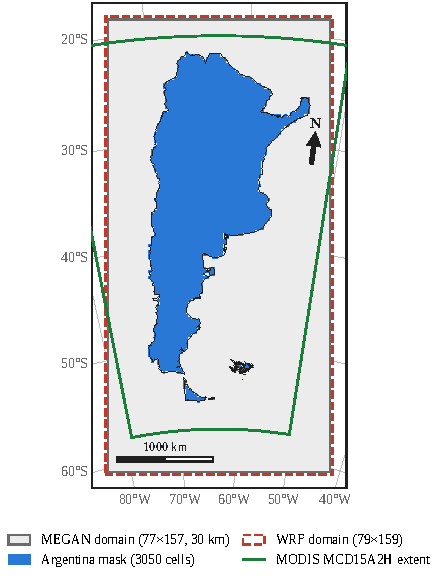
\includegraphics{fig1_domain}
\caption{Simulation domains (30~km Lambert Conformal Conic grid, shown in geographic coordinates): raw WRF domain, trimmed MEGAN domain (30~km), MODIS MCD15A2H download extent, and Argentine land mask (IGN) used to restrict all totals.}
\label{fig:domain}
\end{figure}

In order to capture the seasonal variability of biogenic emissions under contrasting climatic conditions, two representative weeks were simulated: an austral summer week (January 4--10, 2023), corresponding to the period of highest photosynthetic activity and temperature in the region, and an austral winter week (August 1--7, 2023), characterized by lower solar radiation availability and temperatures~\cite{guenther2006,liakakou2007}. This selection allows the sensitivity of the model to the LAI source to be evaluated under two opposing phenological regimes, given that isoprene emissions depend strongly on both active leaf biomass and light and temperature conditions~\cite{guenther1993}.

The updated scenario used LAI derived from MODIS (MCD15A2H product version 6.1, 500~m resolution)~\cite{myneni2021,lin2023}. This product reports LAI values as 8-day composites: for each pixel, the best quality observation available from the Aqua and Terra satellites is selected within a window of 8 consecutive days, dividing the year into 46 fixed periods. The composites corresponding to 2023 that coincide with each simulated week were used (composite 1 for the summer week; composite 27 for the winter week). All other model inputs (canopy type, meteorology, emission factors) were kept constant across all simulations to isolate the effect of the LAI source.

Since the WRF domain extends beyond the political boundaries of Argentina into neighboring countries and the ocean, all reported emission totals and regional statistics were restricted to the Argentine continental territory using a binary land mask derived from official shapefiles from the Instituto Geogr\'afico Nacional (IGN)~\cite{ign}.

To analyze the variation of results according to the ecological region of the country, an ecoregion map~\cite{olson2001,dinerstein2017} was used that divides the territory into zones of similar vegetation and climate (e.g., Chaco, Pampa, Patagonia). Each model grid cell was assigned the corresponding ecoregion based on its geographic location (Fig.~\ref{fig:ecoregions}).

\begin{figure}[!t]
\centering
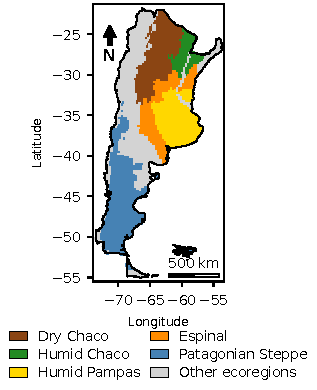
\includegraphics{fig3_ecoregions}
\caption{WWF/Olson terrestrial ecoregions~\cite{olson2001,dinerstein2017} assigned to each 30~km grid cell of the Argentine mask; the number of cells per ecoregion is given in parentheses.}
\label{fig:ecoregions}
\end{figure}

This work presents the accumulation of all estimated emissions for each week of the austral summer and winter seasons. This was done by integrating isoprene emissions over the 24 hours of each day (sum of the 24 hourly time steps), multiplied by 3600~s per hour, for each simulated week.

To compare the impact of the LAI dataset used by default in MEGAN v3.2 (2003, MODIS v4) versus the updated LAI dataset for 2023 (MODIS v6.1) at each grid cell and for each week, the absolute bias,
\begin{equation}
\Delta E = E_{\mathrm{MODIS}} - E_{\mathrm{Default}},
\label{eq:abs}
\end{equation}
and the relative bias over the integrated emission totals,
\begin{equation}
\Delta E(\%) = \frac{E_{\mathrm{MODIS}} - E_{\mathrm{Default}}}{E_{\mathrm{Default}}} \times 100,
\label{eq:rel}
\end{equation}
were calculated, where $E_{\mathrm{MODIS}}$ represents the emissions calculated by MEGAN using the updated LAI dataset for the year 2023 and $E_{\mathrm{Default}}$ the emissions obtained with the standard LAI dataset included within the model.

National and regional totals were calculated by summing these accumulated cell-level emissions within the corresponding spatial subset (Argentina mask or ecoregion polygon).

% ---------------------------------------------------------------------
\section{Results}

In Fig.~\ref{fig:lai} we can observe the spatial distribution of the LAI used in the different scenarios analyzed for the summer and winter seasons. The LAI database used by default in MEGAN, representative of the monthly conditions of the periods of interest from 2003 (produced with MODIS v4 data), is compared with the MODIS version 6.1 LAI product corresponding to 2003 and 2023.

\begin{figure*}[!t]
\centering
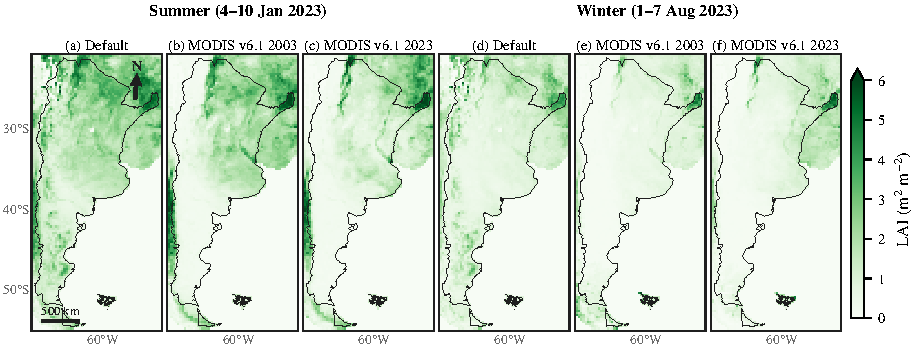
\includegraphics{fig2_lai}
\caption{Spatial comparison of the Leaf Area Index (LAI) over the Argentine continental domain (30~km resolution, Lambert Conformal Conic grid) for the summer (top row; MODIS 8-day composite~1) and winter (bottom row; composite~27) weeks. (a, d) MEGAN v3.2 default LAI climatology (representative of ${\sim}2003$); (b, e) MODIS v6.1 (MCD15A2H) LAI for 2003; (c, f) same for 2023. % VERIFICAR: el pie original decia que el Default estaba corregido por fraccion de cobertura (LAIv->LAI); el array graficado es LAIv/10 sin esa correccion.
 All panels are in LAI units (m$^2$ leaf/m$^2$ ground).}
\label{fig:lai}
\end{figure*}
% VERIFICAR: la version del modelo (antes decia "v3.2.1" en este pie y "v3.2" en el texto).
% VERIFICAR: las etiquetas de fila dentro de la imagen dicen DOY 004-010 y DOY 209-216;
%            conviene unificar el criterio (fechas simuladas vs. composites) al regenerar la figura.

The inclusion of the 2003 MODIS version 6.1 product for both seasons allows the changes associated with the update of the data processing algorithm to be distinguished. Although both MODIS products correspond to the same satellite mission, version 6.1 incorporates a complete reprocessing of the historical archive using improved algorithms, which include refined radiometric calibration, updated atmospheric corrections, improved characterization of observation geometry, more robust quality filters, and advances in the LAI retrieval algorithm~\cite{lin2023}. As a result, the 2003 product in version 6.1 offers a more consistent and accurate LAI estimate than the versions originally used to develop the MEGAN climatology (version 4).

Based on these data, the impact of the update on the national biogenic isoprene emission balance was evaluated. Subsequently, the analysis was extended to the regional scale with the aim of determining whether the sensitivity observed at the national level is homogeneously distributed across the territory or whether, on the contrary, it depends on the characteristics of the vegetation cover and the different ecosystems present in each region.

Table~\ref{tab:national} presents the total sum of weekly ISOP emissions after restricting the simulation domain to the Argentine continental territory using a geographic mask. Emissions were moderately lower when using the updated LAI (MODIS product version 6.1) compared to the standard (Default, i.e., MODIS product version 4), with similar relative differences between seasons: $-2.92\%$ in summer and $-2.86\%$ in winter. However, in absolute terms the difference was considerably larger in summer ($-230\,497$~kmol) than in winter ($-41\,864$~kmol), reflecting that the higher baseline emission load in summer amplifies the absolute effect of the LAI change, even when the relative percentage change is similar between seasons.

\begin{table}[!t]
\centering
\caption{National Weekly Total Isoprene (ISOP) Emissions Restricted to Argentine Continental Territory, Comparing Standard (Default) and Updated (MODIS) LAI Inputs}
\label{tab:national}
\begin{tabular}{@{}lrrrr@{}}
\toprule
Season & \multicolumn{1}{c}{Default} & \multicolumn{1}{c}{MODIS 2023} & \multicolumn{1}{c}{$\Delta E$} & \multicolumn{1}{c}{$\Delta E$} \\
       & \multicolumn{1}{c}{(kmol)} & \multicolumn{1}{c}{(kmol)} & \multicolumn{1}{c}{(kmol)} & \multicolumn{1}{c}{(\%)} \\
\midrule
Summer & \num{7894248} & \num{7663751} & \num{-230497} & $-2.92$ \\
Winter & \num{1462273} & \num{1420409} & \num{-41864}  & $-2.86$ \\
\bottomrule
\end{tabular}
\end{table}

To investigate whether this national pattern was uniform or responded to some regional variable, the results were disaggregated by terrestrial ecoregion, assigning to each grid cell the corresponding World Wide Fund for Nature (WWF)/Olson ecoregion based on its geographic location~\cite{olson2001,dinerstein2017}. This breakdown (Table~\ref{tab:ecoregions}) allowed the relative and absolute sensitivity to be directly compared between ecosystems of different nature within the same analytical framework.

As shown in Table~\ref{tab:ecoregions}, the Dry Chaco, the ecoregion with the highest absolute emissions in the domain (552 cells), showed a moderate and consistent relative sensitivity between seasons ($-2.94\%$ in summer, $-3.84\%$ in winter), in line with the national pattern. The Patagonian Steppe, on the other hand, was the most notable exception in the set: despite having a similar number of cells (584), its total baseline emissions were orders of magnitude lower than those of the Chaco, and its relative sensitivity was considerably higher than the rest of the domain in both seasons, being slightly greater in winter ($-25.1\%$ in summer, $-31.0\%$ in winter). This contrast between an ecoregion of high emission and low relative sensitivity (Chaco) and another of low emission and high relative sensitivity (Patagonia) illustrates that the effect of the LAI change is not distributed proportionally to the size or emissions of each zone, but rather depends on the intrinsic characteristics of each ecosystem. Conversely, the remaining ecoregions, grouped in Table~\ref{tab:ecoregions} as ``Other ecoregions'' ($\sim$10\% of the national total), showed a slight increase in emissions ($+2.6\%$ in summer, $+2.9\%$ in winter), partially offsetting the reductions observed in the main emitting ecoregions.

\begin{table}[!t]
\centering
\caption{Ecoregion-Level Weekly Total Isoprene (ISOP) Emissions for the Summer (S) and Winter (W) Week, Comparing Standard (Default) and Updated (MODIS) LAI Scenarios}
\label{tab:ecoregions}
\setlength{\tabcolsep}{3.2pt}
\begin{tabular}{@{}llcrrrr@{}}
\toprule
Ecoregion & N & & \multicolumn{1}{c}{Default} & \multicolumn{1}{c}{MODIS 2023} & \multicolumn{1}{c}{$\Delta E$} & \multicolumn{1}{c}{$\Delta E$} \\
          &   & & \multicolumn{1}{c}{(kmol)} & \multicolumn{1}{c}{(kmol)} & \multicolumn{1}{c}{(kmol)} & \multicolumn{1}{c}{(\%)} \\
\midrule
\multirow{2}{*}{Dry Chaco}         & \multirow{2}{*}{552} & S & \num{3664145} & \num{3556553} & \num{-107593} & $-2.94$ \\
                                   &                      & W & \num{824486}  & \num{792830}  & \num{-31656}  & $-3.84$ \\
\addlinespace
\multirow{2}{*}{Humid Pampas}      & \multirow{2}{*}{424} & S & \num{1308965} & \num{1266092} & \num{-42873}  & $-3.28$ \\
                                   &                      & W & \num{314578}  & \num{310311}  & \num{-4267}   & $-1.36$ \\
\addlinespace
\multirow{2}{*}{Espinal}           & \multirow{2}{*}{322} & S & \num{1029670} & \num{965923}  & \num{-63747}  & $-6.19$ \\
                                   &                      & W & \num{88081}   & \num{83018}   & \num{-5063}   & $-5.75$ \\
\addlinespace
\multirow{2}{*}{Humid Chaco}       & \multirow{2}{*}{185} & S & \num{1024686} & \num{1013608} & \num{-11079}  & $-1.08$ \\
                                   &                      & W & \num{65914}   & \num{60863}   & \num{-5051}   & $-7.66$ \\
\addlinespace
\multirow{2}{*}{Patagonian Steppe} & \multirow{2}{*}{584} & S & \num{100387}  & \num{75146}   & \num{-25241}  & $-25.14$ \\
                                   &                      & W & \num{2078}    & \num{1434}    & \num{-644}    & $-31.01$ \\
\addlinespace
\multirow{2}{*}{Other ecoregions}  & \multirow{2}{*}{979}  & S & \num{766394}  & \num{786430}  & \num{20036}   & $+2.61$ \\
                                   &                      & W & \num{167135}  & \num{171954}  & \num{4818}    & $+2.88$ \\
\bottomrule
\multicolumn{7}{@{}p{\columnwidth}@{}}{\footnotesize Values are restricted to Argentine continental territory using the IGN-derived land mask. $\Delta E = $ MODIS $-$ Default; $\Delta E(\%) = 100\,\Delta E/$Default. The four main emitting ecoregions are shown, together with the Patagonian Steppe, included as a low-emission, high-relative-sensitivity contrast case. ``Other ecoregions'' is the residual between the national totals (Table~\ref{tab:national}) and the ecoregions listed.}
\end{tabular}
\end{table}
% Verificado con data/ISOP_stats_by_ecoregion_ARGonly_v2.csv: las 4 mayores son Dry Chaco, Humid Chaco,
% Humid Pampas y Espinal en ambas estaciones (5a: Southern Andean Yungas). N total de la mascara = 3046.

The complete spatial distribution of these differences, shown in the maps of relative ($\Delta E\%$; Fig.~\ref{fig:rel}) and absolute biases ($\Delta E$, kmol; Fig.~\ref{fig:abs}), confirms and extends what was observed at the ecoregion level. In relative terms, Patagonian grid cells show a systematic and marked reduction when using MODIS LAI in both seasons (median $\Delta E\%$ of $-33\%$ in summer and $-41\%$ in winter across Patagonian Steppe cells), while the center-north of the country (Chaco, Pampa) presents much more moderate differences, close to zero. The ecoregion-level values in Table~\ref{tab:ecoregions} ($-25.1\%$ and $-31.0\%$) are smaller in magnitude because they are computed from aggregated totals and are therefore weighted toward the higher-emitting cells, where relative changes are less pronounced.
In absolute terms, however, the pattern is markedly seasonal: in summer an intense concentration of negative absolute change is observed in northwestern Argentina (NOA) and the Chaco region (below $-500$~kmol per cell in many cells and locally beyond $-1000$~kmol), while in winter that same zone shows much more subtle absolute changes, practically negligible in the rest of the country. This demonstrates that the relative and absolute sensitivity of the model to the LAI source are not equivalent, nor do they respond in the same way to seasonality: Patagonia is relatively more sensitive to LAI change in both seasons, while the absolute sensitivity of the Chaco/NOA is markedly greater in summer than in winter.

\begin{figure}[!t]
\centering
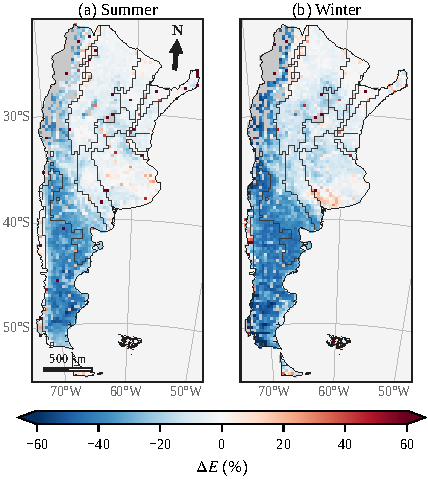
\includegraphics{fig4_rel_bias}
\caption{Relative isoprene emission bias ($\Delta E\%$, MODIS vs.\ Default) for (a) summer and (b) winter, restricted to Argentine territory. The color scale is saturated at $\pm60\%$. Dashed lines: ecoregion boundaries (Fig.~\ref{fig:ecoregions}).}
\label{fig:rel}
\end{figure}

\begin{figure}[!t]
\centering
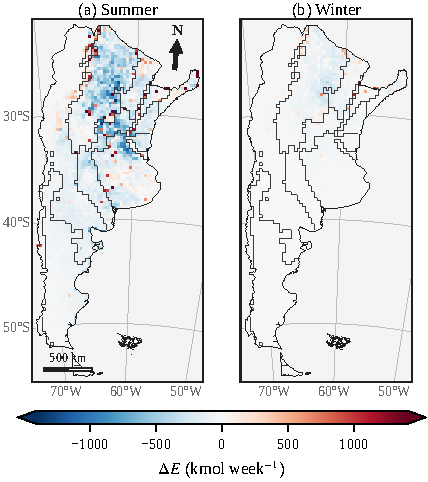
\includegraphics{fig5_abs_bias}
\caption{Absolute isoprene emission bias ($\Delta E = $ MODIS $-$ Default, kmol, weekly total) for (a) summer and (b) winter, restricted to Argentine territory. The color scale is saturated at the 99th percentile of $|\Delta E|$. Dashed lines: ecoregion boundaries (Fig.~\ref{fig:ecoregions}).}
\label{fig:abs}
\end{figure}

Fig.~\ref{fig:temporal} complements the spatial analysis with a temporal characterization of emissions, showing the day-to-day variability within each simulated week (panels a and b) and the mean diurnal cycle (panels c and d).

\begin{figure}[!t]
\centering
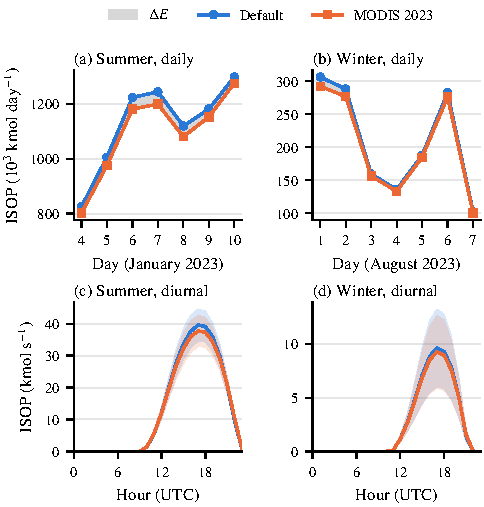
\includegraphics{fig6_temporal}
\caption{Temporal evolution of national isoprene (ISOP) emissions over continental Argentina for the Default and MODIS 2023 LAI scenarios. (a--b) Daily total emissions ($\times10^3$~kmol/day) during the simulated summer and winter weeks; the gray shaded area denotes the emission bias ($\Delta E$) between scenarios. (c--d) Mean diurnal cycle (kmol/s) averaged over the seven simulated days for summer and winter, with shaded envelopes indicating the inter-day standard deviation.}
\label{fig:temporal}
\end{figure}

In terms of daily total emissions (Fig.~\ref{fig:temporal}a and \ref{fig:temporal}b), both scenarios show a very similar temporal evolution in both seasons, with the curves practically overlapping. In summer (Fig.~\ref{fig:temporal}a), daily emissions range between approximately $800\times10^3$ and $1300\times10^3$~kmol/day, with an increasing trend toward the end of the week. In winter (Fig.~\ref{fig:temporal}b), values are considerably lower (between approximately $100\times10^3$ and $310\times10^3$~kmol/day). In both cases, the gap between scenarios (grey area, $\Delta E$) remains constant in relative terms throughout the days, indicating that the sensitivity to LAI does not depend on intra-weekly meteorological variability but rather reflects a structural difference in the LAI input.

The mean diurnal cycle (Fig.~\ref{fig:temporal}c and \ref{fig:temporal}d) shows the characteristic pattern of isoprene emissions controlled by light and temperature~\cite{guenther1993}: zero values during nighttime hours, a marked increase from 10--11~h Coordinated Universal Time (UTC), a peak around 17~h UTC (${\sim}14$~h local time), and a decline toward the late afternoon and evening. In summer, the mean peak reaches ${\sim}40$~kmol/s for the Default scenario and ${\sim}37$~kmol/s for emissions estimated with updated MODIS data; in winter, the peaks are ${\sim}9$ and ${\sim}8$~kmol/s, respectively. The shaded area represents the inter-day standard deviation within each week; although larger in absolute terms in summer, it is proportionally larger in winter, reflecting the greater day-to-day meteorological variability of that week (see also Fig.~\ref{fig:temporal}b). Notably, the shape of the diurnal cycle is practically identical between scenarios, confirming that the effect of LAI acts as a scaling factor on the magnitude of emissions without modifying their temporal distribution.

% ---------------------------------------------------------------------
\section{Discussion and Conclusion}

The results obtained indicate that the LAI source introduces a moderate sensitivity in isoprene emissions simulated by MEGAN for Argentina. Its magnitude, however, is not constant: it varies substantially depending on whether the absolute or relative metric is considered, as well as the region analyzed. The national sensitivity found (${\sim}2.9\%$) was considerably lower than the 29\% reported in~\cite{guenther2006} for changes in the LAI input.

At the national scale, the relative sensitivity did not show a marked seasonality, remaining at similar values between summer and winter ($-2.92\%$ and $-2.86\%$, respectively). Patagonia constituted the main exception to this pattern, with a relative sensitivity systematically higher than the rest of the country in both seasons. The absolute sensitivity, on the contrary, did show a marked seasonal dependence, being considerably greater in summer (particularly in the Chaco). This behavior is consistent with the higher baseline emissions characteristic of that season: the same percentage change in LAI translates into an absolute variation of greater magnitude when the baseline emission is already high~\cite{guenther2006,sun2025}.

This dissociation between absolute and relative sensitivity has a practical implication for the selection of the LAI source, which should be considered according to the objective of each application~\cite{lin2023}. In studies oriented toward the absolute emission balance at the national scale, the LAI update carries greater weight during summer. In contrast, for studies related to the dynamics of Patagonian vegetation, the percentage sensitivity is relevant in both seasons, even when its contribution to the national inventory is marginal given the low baseline emissions of the region.

The present study does not allow determining which of the two LAI data sources more faithfully represents the actual phenology of the vegetation, given that no observations or measurements were available to validate either of the two scenarios~\cite{zhang2004,myneni2021}.

In summary, it is recommended to evaluate both absolute and relative sensitivity when considering the uncertainty associated with LAI in biogenic emission inventories for Argentina, given that both metrics can exhibit different seasonal and regional patterns.

% ---------------------------------------------------------------------
\section*{Acknowledgment}

This work used computational resources from UNC Supercómputo (CCAD) -- Universidad Nacional de C\'ordoba (\url{https://supercomputo.unc.edu.ar}), which are part of SNCAD, Rep\'ublica Argentina. AB thanks CONICET for the PhD fellowship. Financial support from SECYT-UNC and CONICET is acknowledged.

% Igualar columnas en la ultima pagina (pedido de la plantilla IEEE): salto de columna antes de la ref. N.
% Si cambia el texto, ajustar N mirando la ultima pagina.
% \IEEEtriggeratref{N}  % (desactivado: hoy las columnas ya quedan parejas)
\bibliographystyle{IEEEtran}
\bibliography{refs}

\end{document}
